\section*{Instrucciones:}

\begin{itemize}
    \item Entrega en un pdf las respuestas de los ejercicios que no requieran implementarse y añade una breve descripción de los programas que entregas (sus nombres y qué hacen).
    
    \item Los programas deben ir un zip. Debes realizar un programa en cada ejercicio que indique “Implemetar”.

    \item Recuerda que debes utilizar Java 21 LTS.

    \item \textbf{Si no compila utilizando Java 21LTS o si no se entrega la breve descripción de los
    programas se penalizará.}
\end{itemize}

\textbf{Tiempo de elaboración:} $\approx$ 2.5 hrs

\textbf{Total de puntos:} 100

\textbf{Nota:} En esta práctica \textbf{no} es necesario utilizar otros objetos de la biblioteca Concurrent de java que no hayan sido mencionados en el Contexto 1 de esta práctica, por ejemplo: \textit{getAndIncrement, ArrayBlockingQueue, ConcurrentLinkedQueue}. Muchos de estos objetos ya predefinidos en java son implementaciones linealizables: con consistencia, y en esta práctica no lo  necesitamos.

\section*{Ejercicios:}

\begin{enumerate}

\item El programa ColaSecuencial es una implementación de una cola secuencial. Implementa una Cola concurrente utilizando una pool de hilos (ExecutorService). No utilices candados ni synchronized.

\hfill

\item Ejecuta varias veces tu implementación con diferentes secuencias de llamadas a métodos ¿Tu implementación funciona de acuerdo a lo que se espera de una cola o suceden inconsistencias? Por ejemplo,

1) Se hace enq(a), enq(b) y deq() y al final ambos elementos a y b están en la cola.

2) Se realiza un enq(a) y un enq(b) y la cola solo contiene al elemento a o b.

3) Se desencola dos veces el mismo elemento.

Si existe una ejecución así toma una captura pantalla del resultado de tu programa que lo ejemplifique.

\hfill

\textit{Hint: Para analizar si hay inconsistencias, utiliza la interfaz Future, solo ten cuidado con el método get() ya que fuerza a que el resultado del future sea devuelto en ese momento.}

\hfill

\textbf{Importante:} El orden en el que se suben las tareas con submit y se guardan en los futures, no es el orden en el que se realizan, solo es el orden en el que se les asignan a los hilos. Nuestro sistema es asíncrono, es decir, cada hilo puede tardarse más o menos en ejecutar la tarea que se le asignó.

\hfill

\item ¿Existen data races o race-conditions? Explica en qué variables y porqué suceden.

\hfill

\item  Utiliza candados y/o synchronized en tu implementación de forma que los métodos enq() y deq() sean una sola sección crítica y contesta: ¿existen inconsistencias?
Importante: El orden en el que se suben las tareas con submit y se guardan en los futures, no es el orden en el que se realizan, solo es el orden en el que se les asignan a los hilos. Nuestro sistema es asíncrono, es decir, cada hilo puede tardarse más o menos en ejecutar la tarea que se le asignó.

\begin{figure}[h]
    \centering
    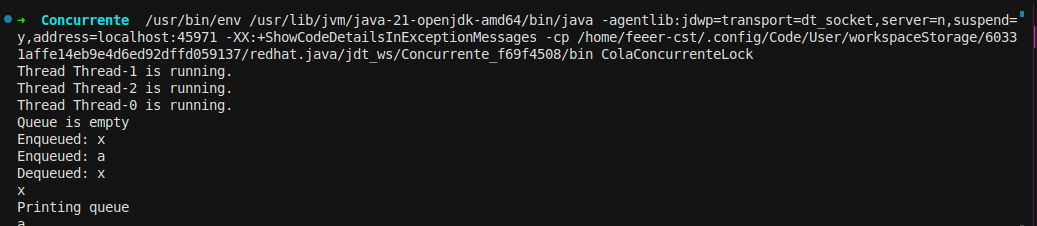
\includegraphics[width=0.8\textwidth]{resources/Ejercicio4.png}
\end{figure}

Podemos ver que no hay inconsistencias, ya que hay locks en la sección crítica donde esto puedo fallar, en especifico el uso de lock()  y unlock() aseguran que un hilo a la vez pueda modificar la cola.
\hfill

\item En una pool de hilos (ExecutorService), ¿si utilizamos más hilos equivale a un mayor throughput?

Argumenta porqué.

\hfill

\item \textbf{Problema.} Supón que perteneces a un equipo de trabajo en el cual estás a cargo de dar acceso a un servidor. Seis personas te pueden mandar tareas para que las ejecutes en el servidor. Las tareas del hilo 0 y 2 tardan 500ns, las del hilo 1 tardan 2000ns y las de los hilos 3, 4 y 5 tardan 3000ns.

Tienes la instrucción de no dar acceso a más de tres al mismo tiempo y de no aceptar al mismo tiempo las tareas del hilo 0 y 2. Diseña e implementa una solución. Hint: Apóyate del programa Scheduler y Tarea, el semáforo inicializado en 3 representa que solo pueden entrar 3 al mismo tiempo, decide como utilizarlo en el programa Tarea (colocando sus métodos adquire y release); además, decide como utilizar un candado, para restringir aceptar las tareas de los hilos 0 y 2 al mismo tiempo.

\begin{itemize}
    \item ¿Tu implementación cumple con Justicia?

    \item Sino es así, describe cómo podrías garantizarla.
\end{itemize}
    
\end{enumerate}
